\documentclass[tikz,border=8pt]{standalone}
% Shared look for every TikZ diagram. Load with % Shared look for every TikZ diagram. Load with % Shared look for every TikZ diagram. Load with \input{../../tools/tikz-style.tex}
\usepackage[T1]{fontenc}
\usepackage{lmodern}
\renewcommand{\sfdefault}{lmr}  % diagrams use the same serif as the text
\usetikzlibrary{arrows.meta, positioning, shapes.geometric, calc, fit, backgrounds}
\definecolor{cblue}{HTML}{4C78A8}
\definecolor{corange}{HTML}{F58518}
\definecolor{cgreen}{HTML}{54A24B}
\definecolor{cred}{HTML}{E45756}
\definecolor{cpurple}{HTML}{B279A2}
\definecolor{cgrey}{HTML}{6B6B6B}
\tikzset{
  every picture/.style={font=\sffamily, line width=1.2pt},
  box/.style={draw=#1, fill=#1!12, rounded corners=4pt, align=center, inner sep=7pt, minimum height=1.1cm},
  box/.default=cgrey,
  arrow/.style={-{Stealth[length=3mm]}, draw=cgrey, line width=1.4pt},
  title/.style={font=\sffamily\bfseries\Large},
  note/.style={font=\sffamily\small, text=cgrey, align=center},
}
\AtBeginDocument{\hyphenpenalty=10000 \exhyphenpenalty=10000}

\usepackage[T1]{fontenc}
\usepackage{lmodern}
\renewcommand{\sfdefault}{lmr}  % diagrams use the same serif as the text
\usetikzlibrary{arrows.meta, positioning, shapes.geometric, calc, fit, backgrounds}
\definecolor{cblue}{HTML}{4C78A8}
\definecolor{corange}{HTML}{F58518}
\definecolor{cgreen}{HTML}{54A24B}
\definecolor{cred}{HTML}{E45756}
\definecolor{cpurple}{HTML}{B279A2}
\definecolor{cgrey}{HTML}{6B6B6B}
\tikzset{
  every picture/.style={font=\sffamily, line width=1.2pt},
  box/.style={draw=#1, fill=#1!12, rounded corners=4pt, align=center, inner sep=7pt, minimum height=1.1cm},
  box/.default=cgrey,
  arrow/.style={-{Stealth[length=3mm]}, draw=cgrey, line width=1.4pt},
  title/.style={font=\sffamily\bfseries\Large},
  note/.style={font=\sffamily\small, text=cgrey, align=center},
}
\AtBeginDocument{\hyphenpenalty=10000 \exhyphenpenalty=10000}

\usepackage[T1]{fontenc}
\usepackage{lmodern}
\renewcommand{\sfdefault}{lmr}  % diagrams use the same serif as the text
\usetikzlibrary{arrows.meta, positioning, shapes.geometric, calc, fit, backgrounds}
\definecolor{cblue}{HTML}{4C78A8}
\definecolor{corange}{HTML}{F58518}
\definecolor{cgreen}{HTML}{54A24B}
\definecolor{cred}{HTML}{E45756}
\definecolor{cpurple}{HTML}{B279A2}
\definecolor{cgrey}{HTML}{6B6B6B}
\tikzset{
  every picture/.style={font=\sffamily, line width=1.2pt},
  box/.style={draw=#1, fill=#1!12, rounded corners=4pt, align=center, inner sep=7pt, minimum height=1.1cm},
  box/.default=cgrey,
  arrow/.style={-{Stealth[length=3mm]}, draw=cgrey, line width=1.4pt},
  title/.style={font=\sffamily\bfseries\Large},
  note/.style={font=\sffamily\small, text=cgrey, align=center},
}
\AtBeginDocument{\hyphenpenalty=10000 \exhyphenpenalty=10000}

\begin{document}
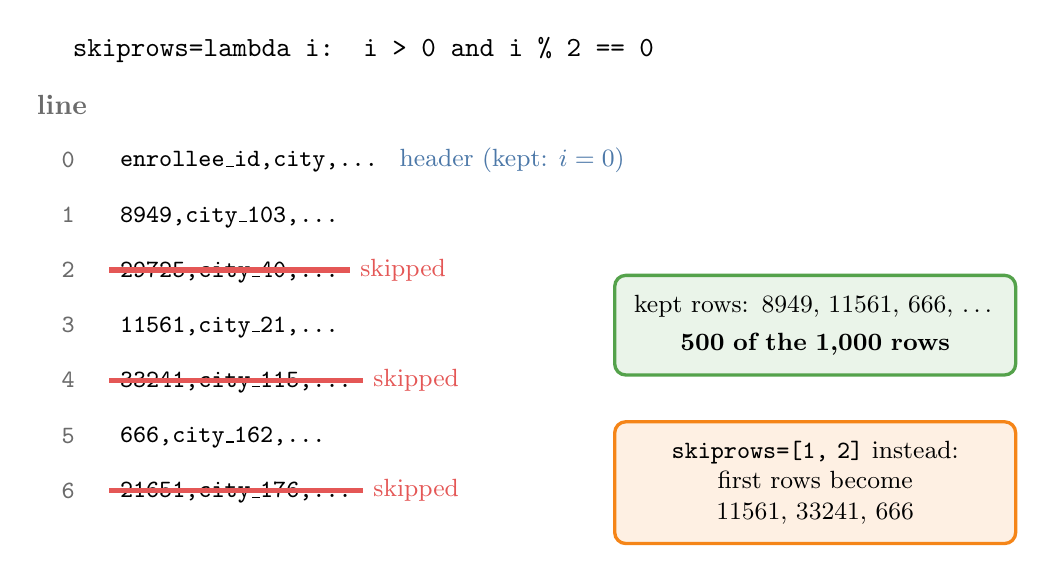
\begin{tikzpicture}[ln/.style={font=\ttfamily\small, text=cgrey, anchor=east},
                    tl/.style={font=\ttfamily\small, anchor=west, text height=1.6ex, text depth=0.4ex}]
  \node[font=\bfseries, anchor=west] at (-0.6,4.9) {\texttt{skiprows=lambda i: i > 0 and i \% 2 == 0}};
  \node[font=\bfseries, text=cgrey] at (-0.6,4.2) {line};
  \foreach \i/\t in {0/{enrollee\_id,city,...}, 1/{8949,city\_103,...}, 2/{29725,city\_40,...}, 3/{11561,city\_21,...},
                     4/{33241,city\_115,...}, 5/{666,city\_162,...}, 6/{21651,city\_176,...}} {
    \pgfmathsetmacro{\y}{3.5-0.7*\i}
    \node[ln] at (-0.3,\y) {\i};
    \node[tl] (t\i) at (0,\y) {\t};
  }
  \foreach \i in {2,4,6} { \draw[cred, line width=2pt] (t\i.west) -- (t\i.east); \node[cred, anchor=west, font=\small] at (t\i.east) {skipped}; }
  \node[cblue, anchor=west, font=\small] at (t0.east) {header (kept: $i = 0$)};
  \node[box=cgreen, anchor=west, text width=4.6cm, font=\small] at (6.4,1.4) {kept rows: 8949, 11561, 666, \dots\\[3pt] \textbf{500 of the 1,000 rows}};
  \node[box=corange, anchor=west, text width=4.6cm, font=\small] at (6.4,-0.6) {\texttt{skiprows=[1, 2]} instead:\\ first rows become 11561, 33241, 666};
\end{tikzpicture}
\end{document}
